\documentclass[twocolumn,amsmath,amssymb,showpacs,prl,superscriptaddress,aps]{revtex4-1}

\usepackage{epsfig}
\usepackage{color}
\usepackage{array}
\usepackage{graphicx}
\usepackage{bm}
\usepackage{epstopdf}


\DeclareMathOperator*{\argmin}{argmin}




\begin{document}




\title{Engineering momentum profiles of cold-atom beams}

\author{D~Hudson \surname{Smith}}
\affiliation{Clemson University, Clemson, South Carolina 29634, USA}

\author{Artem~G \surname{Volosniev}}
\affiliation{Institut f{\"u}r Kernphysik, Technische Universit{\"a}t Darmstadt, 64289 Darmstadt, Germany}


\date{\today}

\begin{abstract}
We ...
\end{abstract}


\maketitle

\section{Introduction}

Scattering is one of the most important observational tools in science. In physics, it is used in almost all subfields to understand internal structure of particles, materials, structures (cite).  

In systems of cold atoms scattering might seem obsolete because the energies are so low that usually only a few parameters determine physics, i.e., the system is in a universal regime. However, even at these low temperatures observables can strongly depend on the incoming momentum (see Figure 1a). For example, ...

{\it Figure 1a: examples where observables depend strongly on the incoming momentum: time-dependent one- and two-body scattering, three-body recombination,  polaron. 
Figure 1b: a sketch of the set-up for engineering beams with desirable momentum profiles: two reservoirs and a link between them.}

Here we study how to create fluxes with cold atoms, which can be used to study systems of cold atoms in scattering experiments. We illustrate using the one-dimensional Bose polaron problem.

\section{Design}

\subsection{Physical System}
Describe the system. The system has three parts: Two reservoirs and a link between them; see Figure 1a. One reservoir is made of a non-interacting (for simplicity) gas of particles at temperature $T$. We call these particles probes or $A$. The reservoir is connected to the link. The link is a potential that acts only on particles $A$ (for simplicity). The second reservoir is made of interacting particles $B$. These particles make a system of interest, which we would like to analyze. 

\subsection{Procedure for Finding a Link Potential}\label{sec:procedure_link}
We find an appropriate link potential $V_0(x) \equiv V(x,\bm{\theta}^*)$ by performing a global search over a family of possible potentials $V(x,\bm{\theta})$ for the parameters $\bm{\theta}^*$ that reduce the difference between the desired transmission-momentum profile $T_0(k)$ and the actual profile $T_{\bm\theta}(k)$ determined by a sample potential $V(x, \bm{\theta})$. Concretely, we minimize the cost $J_{\bm{\theta}}$ which is a function of $T_0(k) - T_{\bm{\theta}}(k)$ but may also explicitly depend upon $V(x,\bm{\theta})$ and $\bm{\theta}$ in order to encode practical, experimental constraints on the solutions for the link potential. Given the cost function, the {\it optimal} parameters are $\bm{\theta}^* = \argmin_{\bm{\theta}}J_{\bm\theta}$. However, we do not need to find the {\it optimal} link potential; one that is {\it good enough} in terms of experimental requirements will do. This relaxed goal alleviates concerns about convergence to the global optimum.

We perform the minimization outlined above using the global optimization routine called Differential Evolution (DE) \cite{original DE paper}. This evolutionary-based search algorithm is suitable given the non-convex (multiple local minima) nature of the optimization problem. Despite its simplicity, DE does a good job of balancing exploration of the space of link potentials against the need to efficiently learn from each sample with little tuning of the model settings. Emperically, we found DE to perform much better than several other approaches including random search, Nelder-Mead, and Simulated Annealing \cite{Tests performed using mathematica}.

We parametrize the family of link potentials $V(x, \bm{\theta})$, as a sum of $N$ Gaussian potentials:
\begin{equation}\label{eq:V-param}
V_N(x,\{\bm{A},\bm{\mu},\bm{\sigma} \}) = \sum_{i=1}^{N}\frac{A_i}{\sqrt{2\pi\sigma_i^2}}\exp\left[{-\frac{(x-\mu_i)^2}{2\sigma_i^2}}\right],
\end{equation}
where $A_j\equiv(\bm{A})_j$, $\mu_j\equiv(\bm{\mu})_j$, and $\sigma_j\equiv(\bm{\sigma})_j$ are the amplitude, mean, and standard deviation for the $j^{\mathrm{th}}$ Gaussian. It is necessary to enforce constraints on these parameters to both improve convergence and to ensure that solutions satisfy the experimental requirements. Table~\ref{tab:constraints} shows the explicit parameter constraints that we enforce  during minimization. 

\begin{table}[t]
  \renewcommand*{\arraystretch}{1.4}
  \begin{tabular}{m{3cm}|m{5.5cm}}
    Constraints & Experimental Rationale \\
    \hline\hline
    $\sum_{i=1}^{N}\mu_i = 0$ & The cost function has a continuous degeneracy associated with overall translations of the link potential. \\
    \hline
    $\sigma_{\mathrm{min}} \leq \sigma_j \leq \sigma_{\mathrm{max}} $ & Laser beam widths fall between a minimum and maximum value.\\
    \hline
    $A_{\mathrm{min}} \leq |A_j| \leq A_{\mathrm{max}}$ & Laser amplitudes fall between a minimum and maximum value.
  \end{tabular}
  \caption{The explicit constraints on the potential parameters and the rationale for each constraint. The values of $\sigma_{\mathrm{min}}$, $\sigma_{\mathrm{max}}$, $A_{\mathrm{min}}$, and $A_{\mathrm{max}}$ must be determined from the experimental context.}
  \label{tab:constraints}
\end{table}

In addition to explicit constraints on the parameters, we inforce an implicit constraint by requireing that the link potential should not extend beyond the region  of potential support $x\in[-x_0,x_0]$. This we do by adding to the cost function a term $J_{\mathrm{boundary}}$ that grows with the area of the potential outside the support region. The complete definition of the cost function is given in suppl.~material. 



 It is clear that by changing the potential in the link we can change the flux. Let us describe how we compute potentials to create desirable fluxes. In this section we discuss this.  Describe the procedure here: We set the desirable momentum profile, guess a potential, calculate the corresponding transmission coefficient, minimize the parameters. 

{\it Figure 2: Examples of a few profiles that can be created: comb, evaporative, anti-evaporative etc. In the insets are the corresponding potentials.}

\section{Illustration}

The Bose polaron problem is very interesting, and many groups are studying it now. It is an open question how to measure the effective mass of the impurity in one-dimensional set-ups. There was one experiment, however the results are unclear. Also it is interesting to understand when the model breaks, i.e., at which momenta. We propose the following experiment: One reservoir -- probes, the link is from Fig. 2 (comb), the second reservoir is an interacting homogeneous Bose gas (for simplicity). Provide some realistic numbers. Probably some simple calculations (in the suppl. material). 

{\it Figure 3: Bose polaron set-up. Measurement of the effective mass -- the change of the energy upon interaction change.}


\section{Summary} 

We have shown how to create beams of particles to probe systems of cold atoms. We have illustrated the idea using the Bose polaron problem. Other interesting examples include ... 

\begin{acknowledgments}
We thank Michael Fleischhauer for referring to~\cite{paper}.
A.~G.~V. gratefully acknowledges the support of the Humboldt Foundation.
\end{acknowledgments}

\widetext

\section{Supplementary Material}

\section{Polaron}

To model one impurity atom that moves through the one-dimensional environment made of $N$ cold bosonic atoms, we employ the following Hamiltonian
\begin{equation}
H=-\frac{\hbar^2}{2m}\sum_{i=1}^N\frac{\partial^2}{\partial x_i^2}-\frac{\hbar^2}{2M}\frac{\partial^2}{\partial y^2}+g\sum_{i>j=1}^N\delta(x_i-x_j)+c\sum_{i=1}^N \delta(x_i-y),
\end{equation}
where $M$ is the mass of the impurity atom, and $m$ is the mass of a bosonic particle. The position of the impurity is $y$, bosons are described by the set of coordinates $\{x_i\}$. 
We assume that the realistic boson-boson and boson-impurity interactions are well-described by the zero-range potentials of strengths $g$ and $c$ respectively. 
The reservoir by assumption is large, such that the dynamics can be described by the thermodynamic limit $N\to \infty$ assuming a certain value of the density $\rho$.
To take the thermodynamic limit we set the periodic boundary conditions: The particles move in a ring of the circumference $L$, such that $0<x_i<L$ and $0<y<L$.
This assumption is not essential for our problem, because we are interested in the limit $N(L)\to \infty$ with $\rho=\frac{N}{L}$.


Every eigenfunction of the Hamiltonian can be written as $\Psi=\sum_{\{n_j\},m} a_{\{n_j\},m}e^{2\pi i \frac{\sum n_jx_j+my}{L}}$. Because all interactions are pairwise, 
the total (angular) momentum of the system must be conserved, and we write it as $P=\frac{2\pi\hbar}{L}\left(\sum_{j} n_j+m\right)$.
Since we have a conserved quantity ($P$), we may exclude the coordinate of the impurity from the consideration. To this end, 
we write the function $\Psi$ as $\Psi=e^{i \frac{P y}{\hbar}}\sum_{\{n_j\},m} a_{\{n_j\},m}e^{2\pi i \frac{\sum n_jz_j}{L}}\equiv e^{i \frac{P y}{\hbar}} \psi(z_1,...,z_N)$ 
with $z_i=L\theta(x_i-y)+x_i-y$, where $\theta(x)$ is the Heavyside step function, i.e., 
$\theta(x>1) = 1$ and zero otherwise. The variables $z_i$ are defined such that $0\leq z_i \leq L$ and the impurity is placed at $z=0$ and $z=L$. Now if we insert this 
function into the Schr{\"o}dinger equation, $H\Psi={\cal E}\Psi$, we obtain the following equation for $\psi(0<z_i<L)$
\begin{equation}
-\frac{\hbar^2}{2m}\sum_i\frac{\partial^2 \psi}{\partial z_i^2}-\frac{\hbar^2}{2M}\left(\sum_{i}\frac{\partial \psi}{\partial z_i}\right)^2
+ i \frac{\hbar P}{M}\sum_{i}\frac{\partial \psi}{\partial z_i}+g\sum_{i>j}\delta(z_i-z_j)\psi=\left({\cal E}-\frac{P^2}{2M}\right)\psi,
\end{equation}
which must be supplemented with the boundary conditions:
\begin{equation}
\psi(z_i=0)=\psi(z_i=L); \qquad \frac{\partial \psi}{\partial z_i}\bigg|^{z_i=0^+}_{z_i=L^-}= \frac{2 c \kappa}{\hbar^2} \psi(z_i=0),
\end{equation}
where $\kappa=mM/(m+M)$ is the reduced mass.

By assumption the bosons are weakly-interacting, therefore we use the ansatz $\psi=\prod_i \Phi(z_i)$ to approximate the function. 
To minimize the expectation value of the Hamiltonian the function $\Phi(z)$ must satisfy the following Gross-Pitaevski-type equation
\begin{equation}
-\frac{\hbar^2}{2\kappa}\frac{\partial^2\Phi}{\partial z^2}+i\frac{\hbar P}{M}\frac{\partial \Phi}{\partial z}
-i \frac{\hbar^2 (N-1) A}{M} \frac{\partial\Phi}{\partial z} + g(N-1)|\Phi|^2\Phi=\mu \Phi,
\end{equation}
where $A=-i\int \Phi(x)^*\frac{\partial}{\partial x}\Phi(x)\mathrm{d}x$ defines the momentum of a boson, and $\mu$ is the chemical potential (it appears as the Lagrange multiplier). 
We rewrite this equation as
\begin{equation}
-\frac{\partial^2\Phi}{\partial z^2}+i v \frac{\partial \Phi}{\partial z} + \tilde g(N-1)|\Phi|^2\Phi+\tilde c\delta(z)\Phi=\tilde\mu\Phi,
\label{eq:GPE_resc}
\end{equation}
where $\tilde\mu=\frac{2 \kappa \mu}{\hbar^2}$, $\tilde g=\frac{2 \kappa g}{\hbar^2}$, $\tilde c=\frac{2 \kappa c}{\hbar^2}$ and 
$v\equiv \frac{2 \kappa P_I}{M \hbar}$, where $P_I=P-\hbar A(N-1)$ defines the momentum of the impurity in the thermodynamic limit.
Note the corresponding boundary conditions 
\begin{equation}
\Phi(z=0)=\Phi(z=L); \qquad \frac{\partial \Phi}{\partial z}\bigg|^{z=0^+}_{z=L^-}= \tilde c \Phi(0),
\end{equation}



This non-linear equation~(\ref{eq:GPE_resc}) has an analytic solution for the soliton-like behavior~\cite{ishikawa1980,hakim1997}, which determines the properties 
of the polaron in our problem. Let us first consider the case with $c=0$. In this case the solution for $v>0$ is
\begin{equation}
\Phi=\sqrt{\frac{\tilde \mu}{\tilde g(N-1)}}\left(1-\beta \mathrm{sech}^2\left[\sqrt{\frac{\tilde\mu\beta}{2}}(z+z_0)\right]\right)^{\frac{1}{2}}e^{i\phi(z)},
\end{equation}
\begin{equation}
\phi(z)=-\pi\theta(z+z_0)+\mathrm{arctan}\left(\frac{\sqrt{\frac{2 v^2}{\tilde \mu}\beta}}{\mathrm{exp}\left[\sqrt{2\tilde \mu\beta}(z+z_0)\right]-2\beta+1}\right),
\end{equation}
where  $\beta=1- v^2/(2\tilde \mu)$, and $z_0$ is some parameter that should be determined from the boundary conditions. It is worthwhile noting that the solution for $v<0$ is $\Phi^*$. We plot this solution in Figs.~\ref{fig:Fig1} and~\ref{fig:Fig2}; for simplicity we consider the region $-L/2<z<L/2$, the region $0<z<L$ easily follows. Note that the solution is not periodic (see $\phi$), however by combining two solution with $\pm z_0$ 
we can construct a periodic solution with a singularity at $z=0$. Therefore, the polaron in this picture is a combination of two moving solitons: The impurity creates a topological defect, which 
leads to a quasiparticle picture. 

%%%%%%%%%%%%%%%%%%%%%%%%%%%%%%%%%%%%%%%%%%%%%%%%%%%%%%%%%%%%%%%%%%%%%%%%%%%%%%%%%%%%%%%%%%%%%%%%%%%%%%%%%%%%%%%%%%%%%%%
\begin{figure}
\centerline{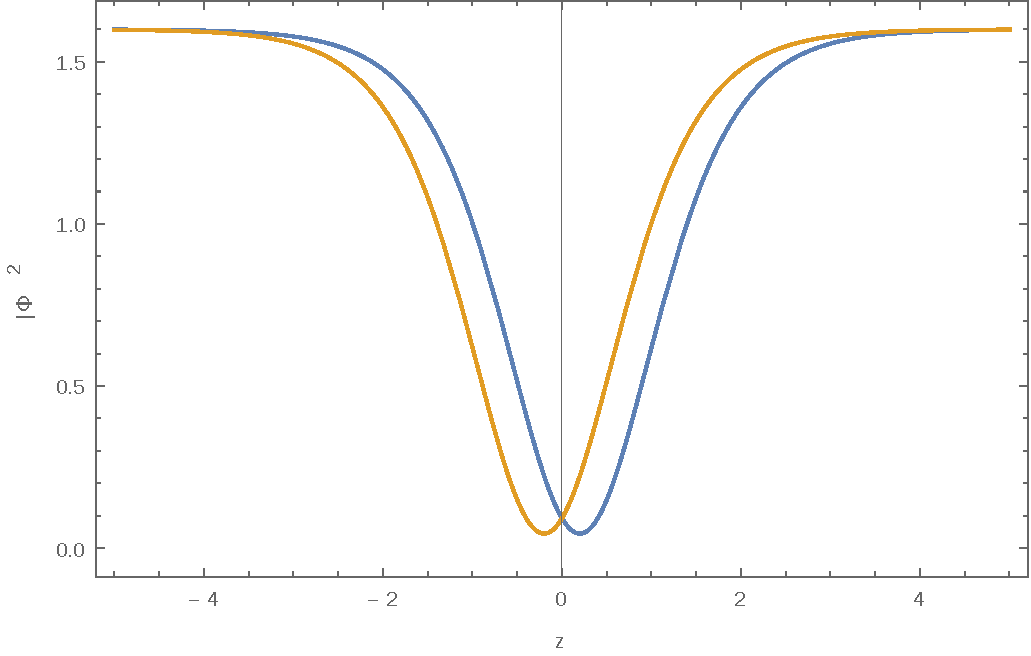
\includegraphics[scale=0.5]{density.pdf}}
\caption{The density, $|\Phi|^2$, of the Bose gas for two different parameters $z_0$: $z_0=0.2$ (left curve), $z_0=-0.2$, assuming that $\tilde \mu=1.6, v=0.3$ (everything in arbitrary units). 
Note that the minimum of the density is at $-z_0$.}
\label{fig:Fig1}
\end{figure}
%%%%%%%%%%%%%%%%%%%%%%%%%%%%%%%%%%%%%%%%%%%%%%%%%%%%%%%%%%%%%%%%%%%%%%%%%%%%%%%%%%%%%%%%%%%%%%%%%%%%%%%%%%%%%%%%%%%%%%%

%%%%%%%%%%%%%%%%%%%%%%%%%%%%%%%%%%%%%%%%%%%%%%%%%%%%%%%%%%%%%%%%%%%%%%%%%%%%%%%%%%%%%%%%%%%%%%%%%%%%%%%%%%%%%%%%%%%%%%%
\begin{figure}
\centerline{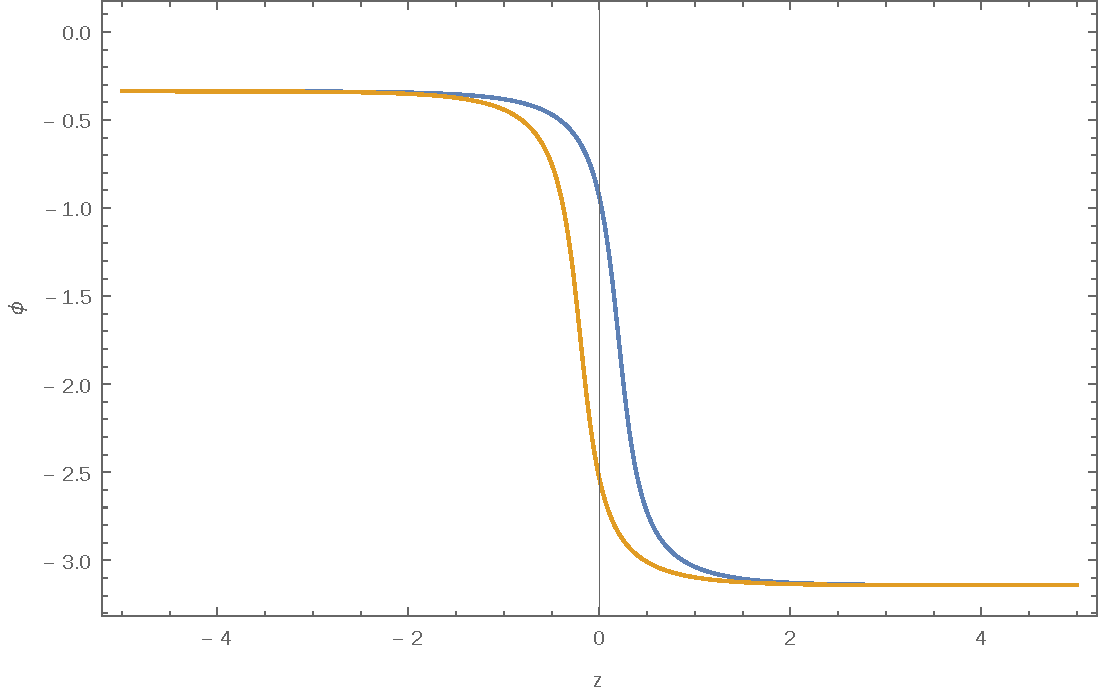
\includegraphics[scale=0.5]{phase.pdf}}
\caption{The phase, $\phi$, of the Bose gas for two different parameters $z_0$: $z_0=0.2$ (left curve), $z_0=-0.2$, assuming that $\tilde \mu=1.6, v=0.3$ (everything in arbitrary units).}
\label{fig:Fig2}
\end{figure}
%%%%%%%%%%%%%%%%%%%%%%%%%%%%%%%%%%%%%%%%%%%%%%%%%%%%%%%%%%%%%%%%%%%%%%%%%%%%%%%%%%%%%%%%%%%%%%%%%%%%%%%%%%%%%%%%%%%%%%%

We write the wave function for the polaron as
\begin{equation}
\Phi=\sqrt{\frac{\tilde \mu}{\tilde g(N-1)}}\left(1-\beta \mathrm{sech}^2\left[\sqrt{\frac{\tilde\mu\beta}{2}}(z\pm z_0)\right]\right)^{\frac{1}{2}}e^{i\phi(z)},
\end{equation}
with 
\begin{equation}
\phi(z)=\delta \phi \theta(-z)+\mathrm{arctan}\left(\frac{\sqrt{\frac{2 v^2}{\tilde \mu}\beta}}{\mathrm{exp}\left[\sqrt{2\tilde \mu\beta}(z\pm z_0)\right]-2\beta+1}\right),
\end{equation}
where the parameter $\delta \phi$ is not important for the further derivations, it reassures that the function is periodic  
(in the thermodynamic limit it is written as $2\pi - \mathrm{arctan}\left[\frac{\sqrt{\frac{2 v^2}{\tilde \mu}\beta}}{1-2\beta}\right]$);
the plus sign in $\pm$ corresponds to $z>0$ and the minus sign to $z<0$. The wave function can be easily visualised from Figs.~\ref{fig:Fig1} and~\ref{fig:Fig2}. 
The density has a non-analytic derivative at $z=0$. The phase is discontinuous function at $z=0$ (the derivative is continuous).



The corresponding chemical potential is found from the normalization condition $\int \Phi^2=1$, for large values of $N$ and $L$ it reads
\begin{equation}
\tilde \mu=\gamma \rho^2 \frac{N-1}{N}\left(1-2\sqrt{2\beta} \frac{ (\mathrm{tanh}(d)-1)}{\sqrt{\gamma}N}\right),
\end{equation}
where $\rho=N/L$, $\gamma=\tilde g/\rho$, and $d=\sqrt{\frac{\gamma \beta}{2}}\rho z_0$.
The condition on $z_0$ is found by using the boundary conditions at $z=\{0,L\}$
\begin{equation}
\frac{\tilde c}{\rho \sqrt{2\gamma}}=\frac{\beta^{\frac{3}{2}}\tanh(d)}{-\beta+\cosh^2(d)}.
\end{equation}
This equation is cubic (in $\tanh(d)$), hence, the solutions can be found in a closed form.
Now we can calculate the energy of the polaron in the thermodynamic limit
\begin{equation}
E\equiv \lim_{N\to\infty, \frac{N}{L}\to \rho}\left[{\cal E}(c,P)-{\cal E}(c=0,P=0)\right],
\end{equation}
where
\begin{equation}
{\cal E}(c,P) = \frac{P^2}{2M} + \mu N-\frac{\hbar^2 A^2 N(N-1)}{2M}-gN(N-1)\int_{0}^{L/2}|\Phi|^4\mathrm{d}z.
\end{equation}
Using these expressions we derive 
\begin{equation}
E=\frac{P_I^2}{2M}+\frac{\hbar^2\rho}{2\kappa}\frac{\sqrt{2 \tilde g \rho \beta}}{3}\left[4 b + (-4b+\beta\mathrm{sech}^2(d))\tanh(d)\right]+\frac{\hbar P_I}{M}\lim_{N\to\infty} A N,
\end{equation}
where $b=1+\frac{v^2}{4\tilde g\rho}=1+\frac{\kappa P_I^2}{2M^2 g\rho}$. This energy for $v\to 0$ can be written as 
\begin{equation}
E\simeq \epsilon+ \frac{P_I^2}{2m_{\mathrm{\mathrm{eff}}}},
\end{equation}
where $\epsilon$ is the effective energy of the polaron, and $m_{\mathrm{eff}}$ is the effective mass.


Further Discussions in the supplementary material and in the paper: 

Discuss the effective mass.

Discuss the two different solutions. 

Discuss the critical momentum. 

Discuss the quench dynamics to the polaron. 

Discuss the literature.

\subsection{Cost Function}\label{sec:cost_function}

\begin{equation}
  J'_{\mathbf{\theta}} = J_{\mathbf{\theta}} + \alpha J_{\mathrm{boundary}},
\end{equation}
where $\alpha>0$ is the weight given to cost incurred for having the potential extend outside the support region of the potential.



\bibliographystyle{apsrev4-1}
\bibliography{bib}

 \end{document}


